\section{Results and discussion}\label{sec:rnd}

\begin{figure}%[h]
\centering
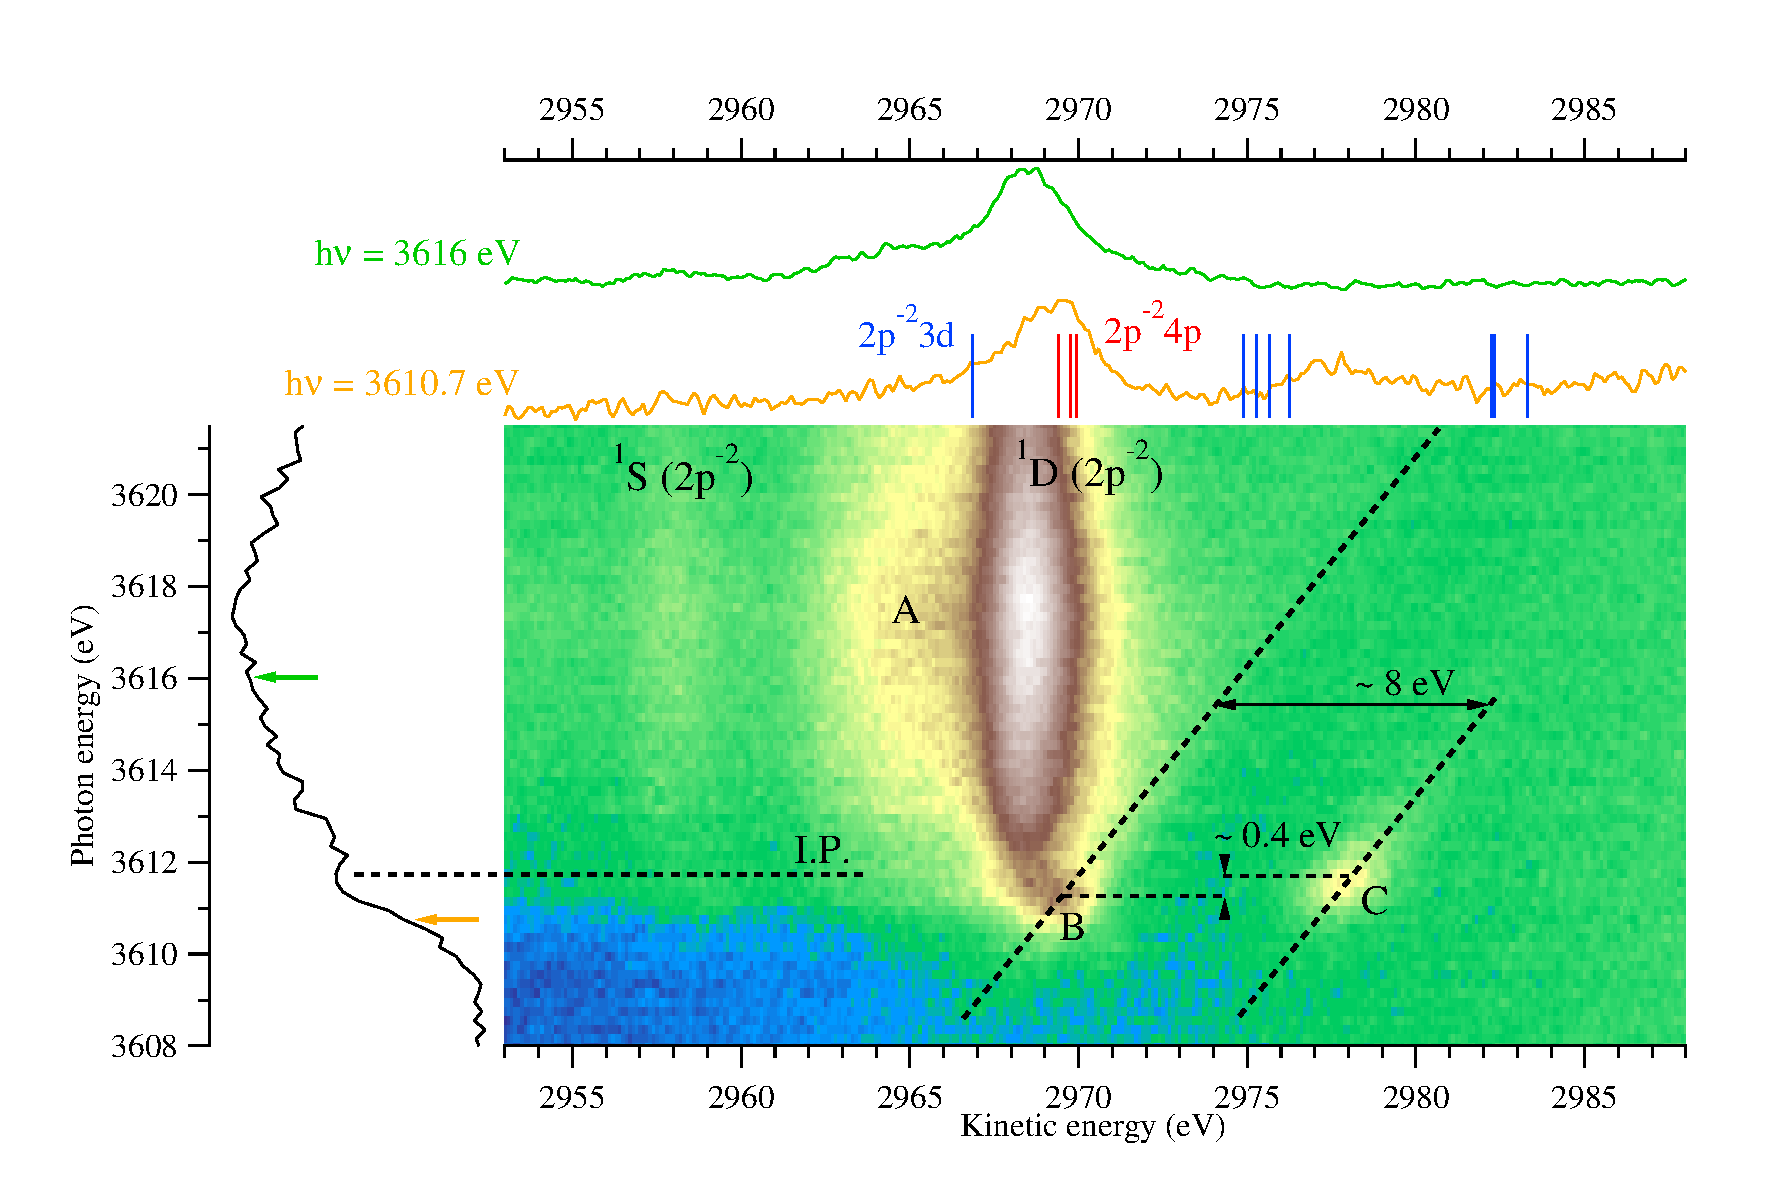
\includegraphics[scale=0.55]{figures/k_2dmap.pdf}
\caption{2D map showing the kinetic energy of the electrons emitted in KL$_{2,3}$L$_{2,3}$ Auger decay vs the photon energy in the vicinity of the K-edge of aqueous K$^{+}$. The black curve on the left represents the experimental partial electron yield spectrum of K$^{+}$ obtained after integrating over the kinetic energies of the Auger electrons in the energy range presented on the figure. The upper panel shows two spectra at photon energies 3610.7\,eV, and 3616\,eV below and above the ionization potential at 3611.9\,eV, respectively. The vertical bars in the resonant Auger spectrum measured at 3610.7\,eV indicate the energy positions of the theoretical final 2p$^{-2}$ 3d (blue) and 2p$^{-2}$4p (red) resonant Auger states of K$^{+}$(H$_2$O)$_6$ of doublet spin multiplicity. The features A, B and C are discussed in the text.}
\label{fg:2dmap_k}
\end{figure}


\begin{figure}%[h]
\centering
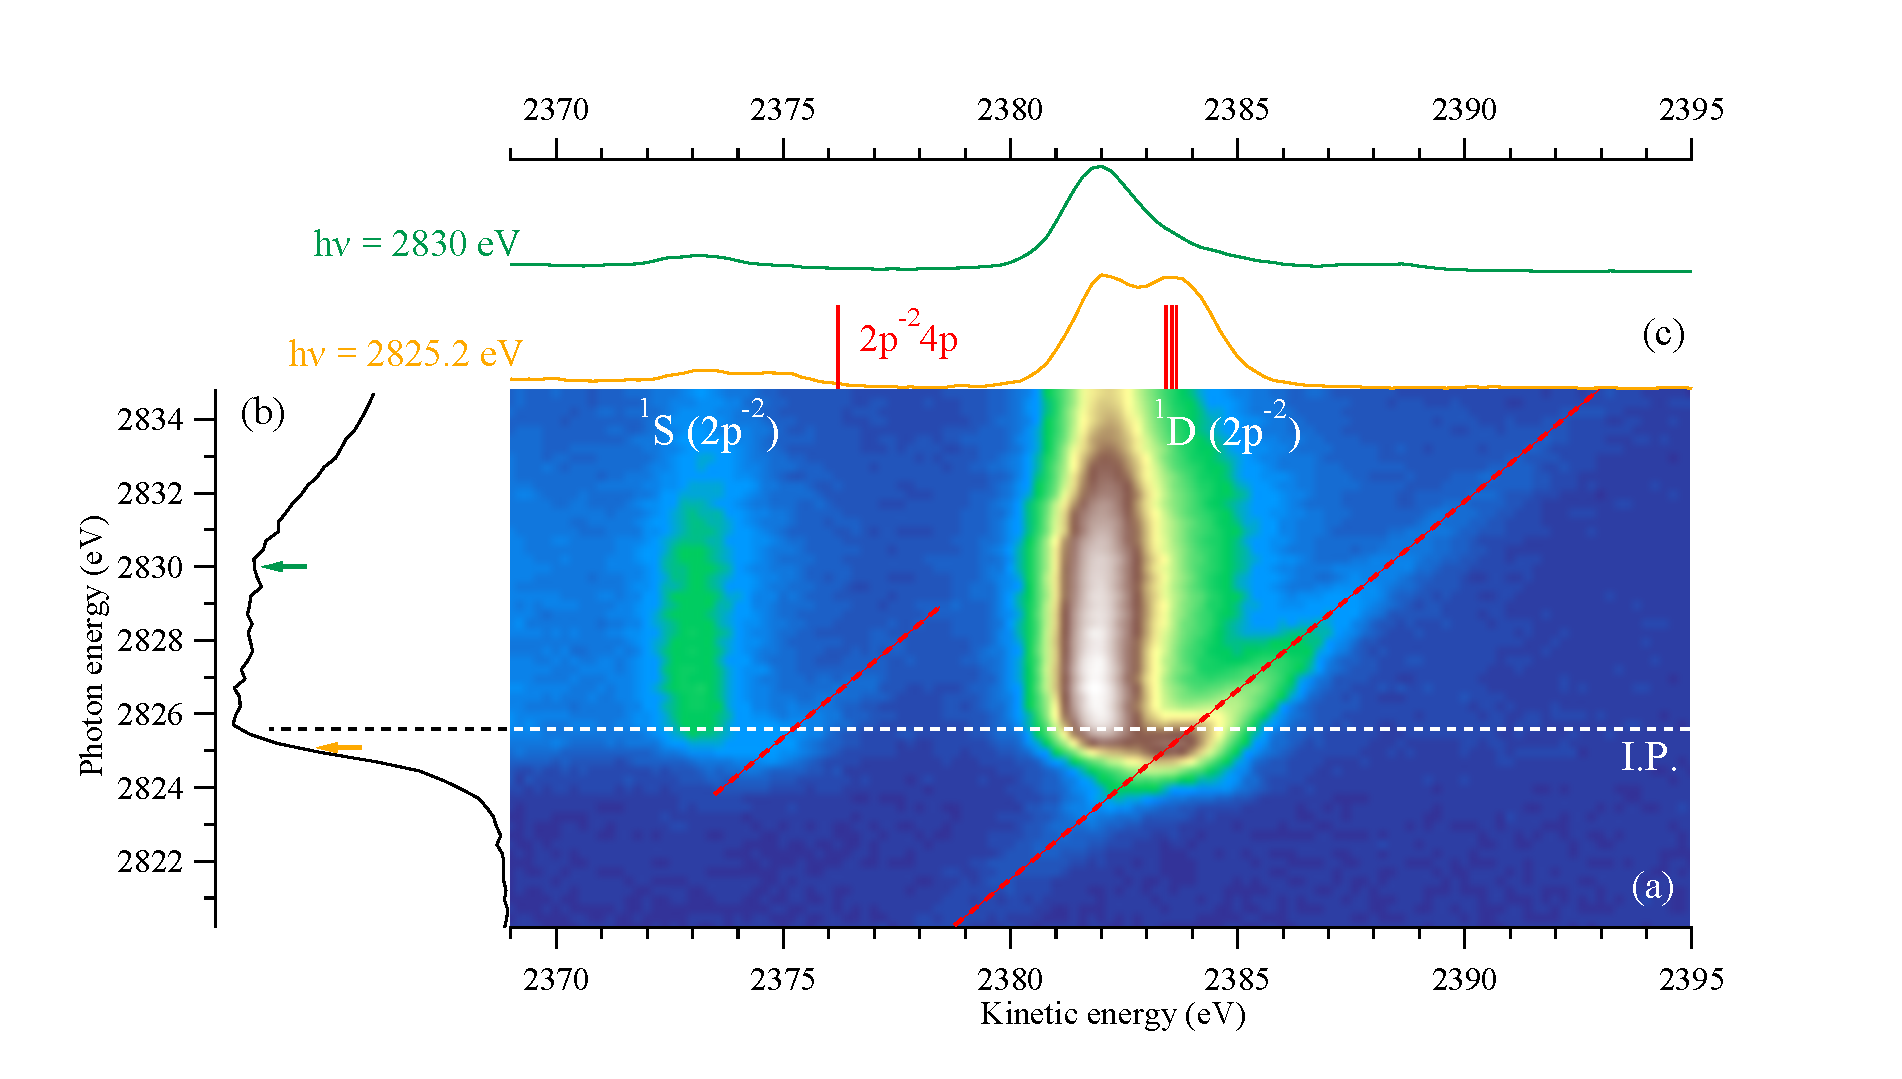
\includegraphics[scale=0.55]{figures/cl_2dmap.pdf}
\caption{2D map showing the kinetic energy of the electrons emitted in KL$_{2,3}$L$_{2,3}$ Auger decay vs the photon energy in the vicinity of the K-edge of aqueous Cl$^{-}$. The black curve on the left represents the experimental partial electron yield spectrum of Cl$^{-}$ obtained after integrating over the kinetic energies of the Auger electrons in the energy range presented on the figure. The upper panel shows two spectra at photon energies 2825.2\,eV, and 2830.0\,eV below and above the ionization potential at 2825.4\,eV, respectively. The vertical bars in the resonant Auger spectrum at 2825.2\,eV indicate the energy positions of the theoretical 2p$^{-2}$4p states of Cl$^{-}$(H$_2$O)$_6$ of doublet spin multiplicity.}
\label{fg:2dmap_cl}
\end{figure}


\subsection{Normal Auger decay}\label{ssec:na}

The KL$_{2,3}$L$_{2,3}$ normal Auger decay following K-shell ionization of aqueous \ki~and \cli~can be written as follows
%
\begin{align*}
h\nu + \text{K}^{+}_{\text{aq}} \rightarrow 
	\text{K}^{2+}_{\text{aq}} (1s^{-1}) + e^{-}_{\text{ph}}\rightarrow
	\text{K}^{3+}_{\text{aq}} (2p^{-2}) + e^{-}_{\text{ph}} + e^{-}_{\text{Auger}}\\
h\nu + \text{Cl}^{-}_{\text{aq}} \rightarrow
	\text{Cl}^{0}_{\text{aq}} (1s^{-1}) + e^{-}_{\text{ph}}\rightarrow
	\text{Cl}^{+}_{\text{aq}}(2p^{-2}) + e^{-}_{\text{ph}} + e^{-}_{\text{Auger}}
\end{align*}
%
It populates the 2p$^{-2}$($^3$P, $^1$D, $^1$S) final states. The $^3$P final states are expected to have a very low intensity since the corresponding transitions are forbidden from angular momentum and parity conservation rules. However, these states are not observed in the experimental spectra presented on Figs.\ \ref{fg:2dmap_k} and \ref{fg:2dmap_cl} because they overlap with the 2p$^{-2}$($^1$D) and 2p$^{-2}$($^1$D)$V'$ states in the kinetic energy region where they are expected to occur. In the case of K$^{+}_{\text{aq}}$ the maxima of the $^1$S and $^1$D KL$_{2,3}$L$_{2,3}$ Auger lines are located at 2958\,eV and 2968.4\,eV, respectively (see Fig.\ \ref{fg:2dmap_k}). For Cl$^{-}_{\text{aq}}$, the lines corresponding to the Cl$^{+}$ 2p$^{-2}$($^1$S) and ($^1$D) states are located at 2373.2\,eV and 2382.1\,eV kinetic energy (see Fig.\ \ref{fg:2dmap_cl}). {\color{red}Which photon energy?}


The KL$_{2,3}$L$_{2,3}$ normal Auger lines may disperse with photon energy close to threshold due to energy exchange between the photoelectron and Auger electron called post-collision interaction (PCI). As a result of this interaction, first, an Auger peak becomes asymmetric with a high kinetic energy shoulder, and second, its intensity maximum is shifted to higher kinetic energies close to threshold \citep{russek86:911,guillemin15:012503}. These effects are seen in our spectra -- the asymmetric tail of the peaks resulting from PCI is clearly shown on the resonant Auger spectra at photon energies 3616\,eV in the case of \ki, and 2830\,eV in the case of \cli.


{\color{red}Gunnar: Including this discussion will invite questions about the energy calibration, and I’m not sure how this was done in these cases. Photoinduced charging may introduce shifts, that can vary with cross section}

Further, we compare the positions of the normal KLL Auger lines of both Cl$^{-}_{\text{aq}}$ and K$^{+}_{\text{aq}}$ close to threshold with those recorded far from threshold, at photon energies $h\nu = 5$\,keV (see Ref.\ \citep{ceolin17:263003} for details). In the latter case, the maxima of the $^1$D and $^1$S states appear at 2381.1\,eV and 2372.3\,eV for Cl$^{-}_{\text{aq}}$, and 2967.4\,eV and 2957\,eV for K$^{+}_{\text{aq}}$, respectively. The maxima were found to be shifted by $\sim$1\,eV towards lower kinetic energies as compared to the spectra measured close to threshold. The magnitude of the shift is constant in the photon energy range of {\color{red}XX\,eV above threshold.} Moreover, it is the same for both ions suggesting that it does not depend on the initial charge of the ion. A possible explanation of the shift observed in our experiment is given in Ref.\ \cite{tchaplyguine07:124314}, which focuses on the Auger decay of large Kr clusters close to the 3d$_{5/2}$ ionization threshold. The observed 4p$^{-2}$($^1$S, $^1$D, $^3$P) Auger peaks were found to be shifted by 0.7\,eV to higher kinetic energies compared to the positions of the peaks far above threshold. Moreover, the shift did not vary with the photon energy close to threshold. Consequently, it was proposed that these features originate from a process of internal ionization, i.e.\ excitation of the photoelectron into the conduction band, followed by normal Auger decay. The observed shift was explained as resulting from the PCI-like interaction between the electron excited in the conduction band and the Auger electron. Further investigations are, however, planned in the case of liquid samples.


Finally, the normal Auger $^1$D main line of K$^{+}$ differs from that of Cl$^{-}$ by the presence of a large shoulder (feature A on Fig.\ \ref{fg:2dmap_k}) on the low kinetic energy side at about 2965\,eV kinetic energy. This shoulder is attributed to electron transfer from the solvent water molecules to the unoccupied 3d orbitals of K$^{+}$ \citep{ceolin17:263003}. In the case of \cli, there is no experimental evidence of such intense electron transfer processes.


\subsection{Resonant Auger decay} \label{ssec:ra}

%\kolya{XAS of Cl- and K+ from previous works?}

The KL$_{2,3}$L$_{2,3}$ Auger decay following resonant K-shell excitation of solvated \ki~and \cli~can be written as follows
%
\begin{align*}
h\nu + \text{K}^{+}_{\text{aq}} \rightarrow \text{K}^{+*}_{\text{aq}} (1s^{-1}V) \rightarrow \text{K}^{2+}_{\text{aq}} (2p^{-2}V') + e^{-}_{\text{Auger}}\\
%
h\nu + \text{Cl}^{-}_{\text{aq}} \rightarrow \text{Cl}^{-*}_{\text{aq}} (1s^{-1}V) \rightarrow \text{Cl}^{0}_{\text{aq}}(2p^{-2}V') + e^{-}_{\text{Auger}}
\end{align*}
%
where $V$ and $V'$ denote the unoccupied orbitals in the presence of the 1s$^{-1}$ and 2p$^{-2}$ core holes, respectively. The character of these states is discussed below.

The pre-edge regions of the x-ray absorption spectra of \ki~and \cli~shown in the left panels of Figs.\ \ref{fg:2dmap_k} and \ref{fg:2dmap_cl} do not exhibit any high intensity peaks owing to the lifetime broadening and energetic proximity of the core excited states to the ionization threshold. Consequently, solely from these absorption spectra, one cannot conclude whether there are core excited states in the pre-edge structure. Instead these states have to be identified by their resonant Auger features which differ from the normal Auger features of core ionized states. Thus, for \cli, the lowest core excited state is located at 2825.2\,eV, which agrees very well with the position of the Cl$^{-}$ 1s$\,\rightarrow\,$4p excitation determined from Cl K-edge XAS experiments in MgCl$_2$.6H$_2$O and of SrCl$_2$/SrCl$_2$.6H$_2$O \citep{sugiura82:681} and MCl$_{4}^{-}$ compounds \citep{shadle95:2259}. In the case of \ki, there are two dispersive features with maxima at photon energies of 3611.2\,eV (B) and 3611.6\,eV (C), respectively (Fig.\ \ref{fg:2dmap_k}). The positions of these two core excited states are close to the energy of the 1s$^{-1}$4p excitation in bare \ki~at 3610.7\,eV \citep{hertlein06:062715}.


The resonant Auger features produced in the decay of these core excited states are quite different for \cli~and \ki. In the 2D map of \cli~shown in Fig.\ \ref{fg:2dmap_cl} there are two dispersive features, indicated with diagonal dashed lines, each on the high kinetic energy side of the $^1$S and $^1$D main lines. The maxima of these features are at 2825.2\,eV photon energy and 2374.6 and 2383.4\,eV kinetic energy, respectively. In the case of \ki (see Fig.\ \ref{fg:2dmap_k}), the dispersive line related to the $^1$S main line cannot be clearly identified due to the presence of strong background. Instead two dispersive features related to the $^1$D main line are observed (features B and C indicated with diagonal dashed lines on Fig.\ \ref{fg:2dmap_k}). Feature B exhibits a maximum at $h\nu = $3611.2 \,eV and 2969.2 \,eV kinetic energy. The additional feature C appears as a separate island away from the main lines on the 2D map of \ki. It is located at $h\nu = $3611.6\,eV and 2978.1\,eV kinetic energy, thus it is separated by approximately 400\,meV in photon energy and 8.3\,eV in kinetic energy from the maximum of feature B. 

\begin{figure}[h!]
\centering
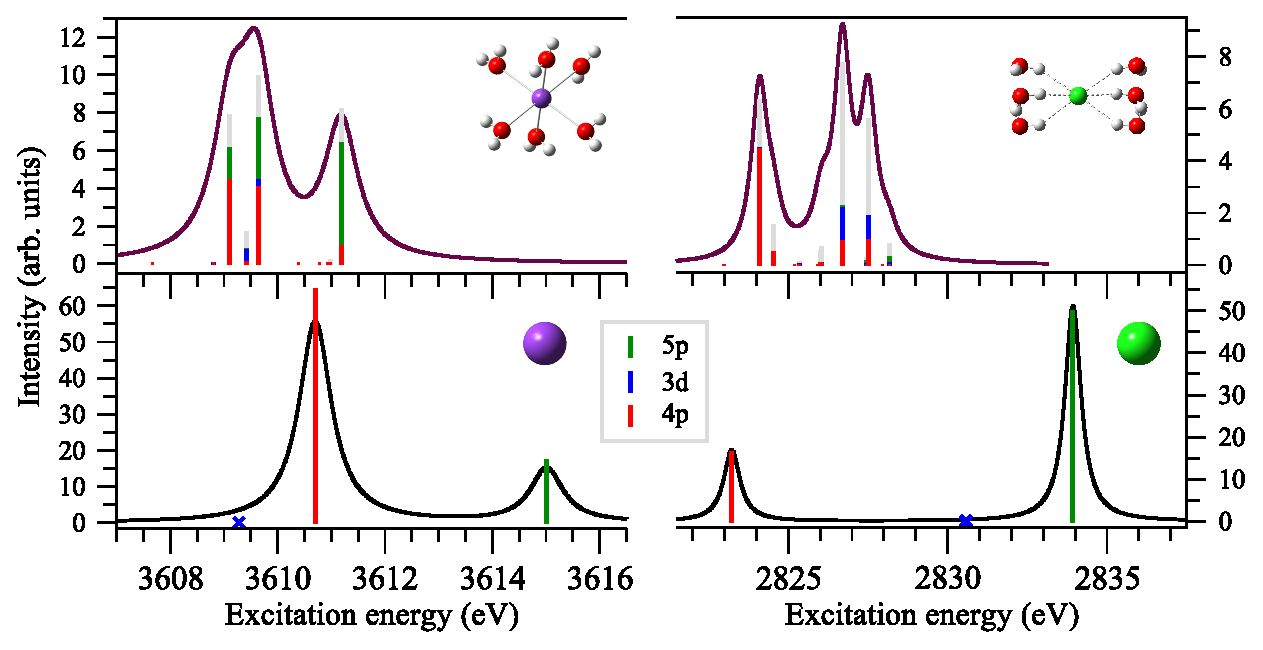
\includegraphics[scale=0.8]{figures/xas_spectra.eps}
\caption{XAS spectra of the lowest K-shell resonant transitions in the bare K$^{+}$ (lower left panel) and Cl$^{-}$ (lower right panel) ions and their 6-coordinated clusters (upper left panel, \ki(H$_2$O)$_6$, and upper right panel, \cli(H$_2$O)$_6$). The theoretical stick spectra were convolved with a Lorentzian profile of FWHM 0.74\,eV for \ki~and 0.62\,eV for \cli~(dashed line)\citep{ceolin17:263003} and a Voigt profile to account for the lifetime broadening and the experimental resolution (full line). The stick spectrum corresponds to the projections $|a_{nl}^{i}|^2$ of the SONOs corresponding to the core excited states of the 6-coordinated clusters on the basis of SONOs corresponding to the 1s$^{-1}$3d, 1s$^{-1}$4p, and 1s$^{-1}$5p states in the bare K$^+$ and \cli~ions (Eq.\ \ref{eq:sono_proj}). The grey sticks in the stick spectrum correspond to contributions from higher-lying atomic core excitations or from excitations to the solvent molecules. The theoretical XAS spectra of both \ki~and \cli~were shifted to higher photon energies such that the excitation energies of the lowest core excited states correspond to the experimentally determined energies -- 3610.7\,eV in the case of \ki, and 2825.2\,eV in the case of \cli. The experimental ionization thresholds are depicted as grey boxes starting at photon energies of 3611.9\,eV (\ki$_{\text{aq}}$) and 2825.4\,eV (\cli$_{\text{aq}}$).}
\label{fg:xas_kcl}
\end{figure}


In order to rationalize the pre-edge region of the experimental XAS spectra and the differences in the AES spectra of \ki$_{\text{aq}}$ and \cli$_{\text{aq}}$, we computed the lowest core excited states of the bare \ki~and \cli~ions and their hexa-coordinated clusters. The theoretical XAS spectra are presented in Fig.\ \ref{fg:xas_kcl}. In the bare ions (lowermost panels on Fig.\ \ref{fg:xas_kcl}), the lowest energy peak corresponds to the dipole allowed 1s$^{-1}$4p state. The next dipole allowed state, 1s$^{-1}$5p, is located 4.3\,eV and 10.8\,eV higher in the cases of \ki~and \cli, respectively. Together with the two dipole allowed transitions, we show the dipole forbidden 1s$^{-1}$3d states of the bare ions as blue crosses at photon energies 3611.17\,eV in the case of \ki~and 2831.68\,eV in the case of \cli, respectively. It is noteworthy that the positions of the 1s$^{-1}$4p and 1s$^{-1}$3d states are inverted in \ki~and \cli. In the case of Cl$^{-}$ the 1s$^{-1}$4p excitation has lower energy and the 1s$^{-1}$3d excitation is close to the 1s$^{-1}$5p state. On the contrary, in K$^{+}$ the 1s$^{-1}$3d excitation has lower energy and lies below the 1s$^{-1}$4p state. We note in passing that the intensity of the Cl$^{-}$(1s$^{-1}$4p) state is lower than that of the \cli(1s$^{-1}$5p) state contrary to what is observed in \ki. This difference can be explained by the lower electron density of the 4p compared to the 5p electron in the region close to the core hole which thus results in the lower oscillator strength of the 1s$^{-1}$4p compared to the 1s$^{-1}$5p transition in \cli~(see Fig.\ \ref{fg:si_rdens_ions} in SI).


The water molecules in the first solvation shell have several effects on the core excited states. First, upon addition of water molecules, the degeneracy of the 1s$^{-1}$4p state is lifted and the intensity of the resulting states in the cluster drops. Moreover, the character of these states changes as can be seen on the upper panels of Fig.\ \ref{fg:xas_kcl}. They are no longer of pure atomic character but they rather interact with states of the neighboring water molecules (shown as grey bars in Fig.\ \ref{fg:xas_kcl}) and with other closely lying states of the bare ion, such as the dipole allowed 1s$^{-1}$5p and dipole forbidden 1s$^{-1}$3d state. Thus, the latter also acquire intensity in the cluster due to mixing with the dipole allowed states in the ligand field of the solvent. A similar effect was observed in the XAS spectra of microsolvated clusters of Na$^{+}$ and Mg$^{2+}$ \citep{miteva16:16671}.


Further we assume that only the lowest peak in the theoretical XAS spectra is populated in the experiment for two reasons. First, due to the lifetime broadening, it spreads over approximately 2\,eV which coincides with the width of the pre-edge structure in the experimental XAS spectra. Second, the splitting between the first core excited state and the ionization threshold in the experiment is 1.2\,eV for \ki~and 0.2\,eV for \cli, and thus it is smaller than the splitting between the first and second peak in the theoretical spectra (1.5\,eV for \ki~and $\sim$3\,eV for \cli, Fig.\ \ref{fg:xas_kcl}). In the 6-coordinated cluster (Fig.\ \ref{fg:xas_kcl} upper left panel), which represents the complete first solvation shell around \ki, the lowest peak in the spectrum contains three states. The lowest and highest lying states are split by approximately 0.5\,eV and they have mixed 4p and 5p character. The low intensity state in between these two states has a predominantly 1s$^{-1}$3d character. Since the dispersive feature B appears at lower excitation energies compared to the feature C, we assume that it is produced in the resonant Auger decay of the lowest core excited states of \ki, which are predominantly of 1s$^{-1}$4p character. Moreover, we can attribute the feature C to the resonant Auger decay of the low intensity dipole forbidden 1s$^{-1}$3d state. Thus, we explain both the energy splitting of $\sim$400\,meV photon energy of the two features, and the fact that island C has lower intensity than feature B (Fig.\ \ref{fg:2dmap_k}).


In the hexa-coordinated cluster of \cli, the solvent molecules have little influence on the position and character of the first state. Due to the large energy separation from other \cli~states it has mainly \cli~1s$^{-1}$4p character with some admixture of states of the nearest water molecules. We therefore attribute the two dispersive features associated with the $^1$S and $^1$D main lines on the 2D map of \cli~to the resonant Auger decay of this core excited state involving mostly the 4p orbitals of chloride.


To fully characterize the dispersive features on the experimental 2D maps, we also computed the lowest K$^{2+}$[2p$^{-2}$nl](H$_2$O)$_6$ and Cl$^{0}$[2p$^{-2}$nl](H$_2$O)$_6$ states of the hexa-coordinated clusters corresponding to the lowest final spectator resonant Auger states. The energy positions of these lines are shown as bars on the experimental resonant Auger spectra in the upper panels of Figs.\ \ref{fg:2dmap_k} and \ref{fg:2dmap_cl}. In both cases, we shifted the lowest 2p$^{-2}$($^1$D)4p states such that the kinetic energies coincide with the maxima of the dispersive features on the high kinetic energy part of the $^1$D main line. Note that we only indicate resonant Auger transitions to the spin-allowed final states of doublet multiplicity. Since the initial core excited states are populated by photon excitation, only doublet states are efficiently populated in the resonant Auger decay. The energetic positions of the 2p$^{-2}$nl states of \ki(H$_2$O)$_6$ and \cli(H$_2$O)$_6$ are substantially different, reflecting the fact that the 3d unoccupied orbitals of \ki~are lower than the 4p orbitals. This is the opposite of what is observed in \cli, where the 2p$^{-2}$3d states (not shown) are located on the lower kinetic energy side of the respective 2p$^{-2}$4p states.


As mentioned above, we attribute the island B to the decay of the lowest lying core excited state, which has predominantly 1s$^{-1}$4p character. Supposing that this state undergoes mostly pure spectator resonant Auger decay, which is the case of the 1s$^{-1}$4p state in the isoelectronic Ar atom \citep{ceolin15:022502}, then the lowest states of 2p$^{-2}$4p character are populated resulting in resonant Auger lines located between 2969 and 2970.5\,eV. As can be seen from the Auger electron spectrum at $h\nu = 3610.7$\,eV (upper panel of Fig.\ \ref{fg:2dmap_k}), the lowest 2p$^{-2}$4p states of \ki(H$_2$O)$_6$ starting at electron energy of 2969\,eV are separated by $\sim$5 and 12-13\,eV from the two groups of 2p$^{-2}$3d states located at higher electron kinetic energies. Thus, the group of 2p$^{-2}$3d states at $\sim$2975\,eV lies closer to the position of island C. Consequently, we attribute this dispersive feature as originating from the resonant Auger decay of the 1s$^{-1}$3d excitation to the group of 2p$^{-2}$3d states lying around 2975\,eV. The splitting between the 2p$^{-2}$4p and 2p$^{-2}$3d states in our calculation is smaller than the splitting between the islands B and C. This difference may be due to the fact that we do not account for the effect of distant solvent shells in our calculation. Concerning the higher lying group of 2p$^{-2}$3d states at kinetic energies between 2982 and 2983\,eV, we conclude that these states are not populated via the Auger process since no additional experimental features are observed.


The energy difference between the spectral features A and C provides another argument in favor of the 2p$^{-2}$ 3d character of the feature C. The feature A originates from electron transfer processes from water molecules (W) to the doubly core ionized potassium ion and has the configuration K$^{2+}$(2p$^{-2}$3d)W$^{-1}$. The lowest ionization potential of liquid water in the liquid phase is about 11.16\,eV \cite{winter04:2625} which fits well with the observed A-C splitting. Based on the above energetic arguments we attribute the island C as originating from resonant Auger decay to the K$^{2+}$ 2p$^{-2}$3d final state.


In the computed Cl$^{0}$[2p$^{-2}$nl](H$_2$O)$_6$ spectrum there are two groups of states split by about 7\,eV (see upper panel of Fig.\ \ref{fg:2dmap_cl}). The lower kinetic energy group corresponds to the 2p$^{-2}$($^1$S)4p final states, whereas the higher kinetic energy group corresponds to the 2p$^{-2}$($^1$D)4p final states. The splitting between these two groups is in good agreement with the experimental splitting between the dispersive features on the high kinetic energy sides of the $^1$S and $^1$D main peaks. Consequently, we attribute these dispersive features as resulting from the resonant Auger decay of the 1s$^{-1}$4p core excited state of \cli$_{\text{aq}}$ to the 2p$^{-2}$($^1$S)4p and  2p$^{-2}$($^1$D)4p final states. Similar dispersive features originating from the decay of the Cl (1s$^{-1}$4p) state were observed on the 2D map of chloromethane CH$_3$Cl recorded in the vicinity of the Cl K-edge in gas phase \cite{gold16:133001}. In this case, however, additional lower-lying core excited states are observed. They result from excitation to the LUMO of CH$_3$Cl, which is a linear combination of the C 2p and Cl 3p atomic orbitals. Since the 3p shell is fully occupied in \cli, such core excited states are not observed in our experiment. We note that neither 2p$^{-2}$3d nor charge transfer states are found in the Cl$^{-}_{\text{aq}}$ case.


\subsection{Delocalization vs resonant Auger decay}

As mentioned above, the delocalization of core excited electrons in aqueous solutions is ultrafast and as such it competes with the resonant Auger decay. In order to estimate the delocalization rate of the core excited electron at the pre-edges of \ki~and \cli, we used the core-hole clock method \cite{bjorneholm92:1892,karis96:1380}.

In the case of \cli, it was possible to perform the same data treatment as in Ref.\ \cite{ceolin15:022502} i.e., for each photon energy step, all components of the 2D map shown in Fig.\ \ref{fg:2dmap_cl} were isolated by fitting procedures and their intensity integrated to get a partial electron yield as a function of the photon energy. The result is shown on Fig.\ \ref{fg:si_ct_time} in the SI. The figure shows that there is a large overlap between the resonant and normal Auger contributions, due to the proximity of the resonance to the ionization potential and due to the very short lifetime of the corresponding states. At the specific photon energy corresponding to the lowest core excitation, $h\nu = 2825.2$\,eV (Fig.\ \ref{fg:2dmap_cl}, upper panel) a double-peak structure is observed in the interval of kinetic energies 2380 -- 2385\,eV . The position of the first peak coincides with the $^1$D main line resulting from normal Auger decay, whereas the second peak at 2383.5\,eV corresponds to the resonant Auger decay to the 2p$^{-2}$($^1$D)4p states. By fitting this double-peak structure with two Voigt functions, we determine the ratio of the intensities of these peaks to be $l/d \approx 1$. From the ratio $l/d$ and the Auger lifetime $\tau_{\text{c}}$, one can determine the delocalization time $\tau_{\text{CT}}$ according to the relation $\tau_{\text{CT}} = \tau_{\text{c}}l/d$ \citep{foehlisch05:373}{\color{red}MORE REFS}. Consequently, the delocalization time $\tau_{\text{CT}}$ is of the same order as the Auger lifetime, i.e.\ $\sim$1\,fs. The fast delocalization in this case is a result of the fact that the energy splitting between the \cli~(1s$^{-1}$4p) resonance and the ionization threshold is 0.2\,eV, and thus, smaller than the lifetime broadening of 0.62\,eV \citep{ceolin17:263003}.


For potassium, the treatment is more complex due to the presence of multiple simultaneous processes -- normal, resonant Auger decay, charge transfer from solvent. To extract the intensity of each component from the 2D map shown in Fig.\ \ref{fg:2dmap_k}, one needs the spectral fingerprints of each process to be separated. However, as can be seen, this is hardly possible especially close to threshold in the kinetic energy region 2965 -- 2970\,eV. For instance at 3610.7\,eV photon energy on the high-kinetic-energy side of the $^1$D main line, there are contributions from the PCI tail and from the 2p$^{-2}$($^1$D)4p resonant Auger state. On the low-kinetic-energy side, the charge transfer processes lead to a very large structure whose shape unfortunately cannot be easily simulated by a known profile. However, the lifetime of the 1s core hole is shorter for potassium than for chloride (0.9 vs.\ 1\,fs) and, moreover, the core excited state appears 1.2\,eV below the ionization threshold whereas it is only 0.2\,eV for chloride. Therefore, one can expect much less efficient delocalization compared to \cli$_{\text{aq}}$.